\documentclass[tikz,border=2pt]{standalone}
\usepackage{amsmath,amssymb}
\usepackage{tikz}
\usetikzlibrary{arrows.meta}

\begin{document}
% An unbounded LP: the feasible region extends forever in an improving direction, so the
% objective lines can be pushed out without limit.
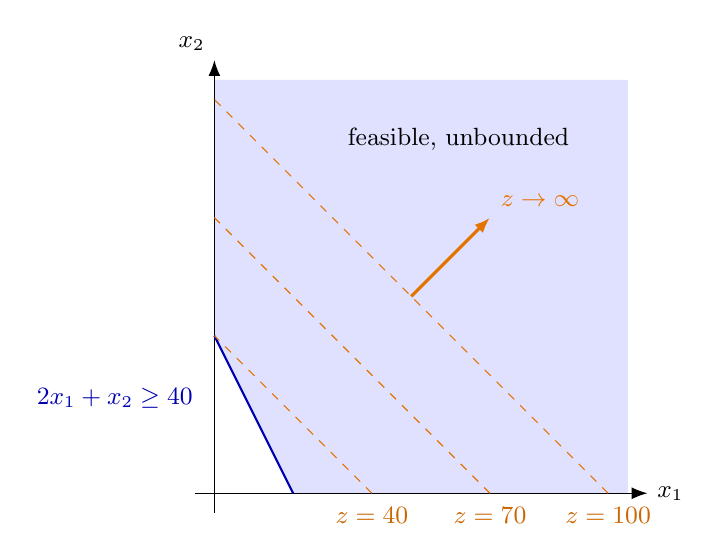
\begin{tikzpicture}[x=0.05cm, y=0.05cm, every node/.style={font=\small}, >={Latex[length=2mm]}]
	\fill[blue!12] (20,0) -- (105,0) -- (105,105) -- (0,105) -- (0,40) -- cycle;
	\draw[->] (-5,0) -- (110,0) node[right] {$x_1$};
	\draw[->] (0,-5) -- (0,110) node[above left] {$x_2$};
	\draw[blue!70!black, thick] (20,0) -- (0,40);
	\node[blue!70!black, font=\small, anchor=east] at (-3,24) {$2x_1+x_2\ge40$};
	\draw[orange!90!black, dashed] (40,0) -- (0,40);
	\draw[orange!90!black, dashed] (70,0) -- (0,70);
	\draw[orange!90!black, dashed] (100,0) -- (0,100);
	\node[orange!80!black, font=\small, anchor=north] at (40,-1) {$z=40$};
	\node[orange!80!black, font=\small, anchor=north] at (70,-1) {$z=70$};
	\node[orange!80!black, font=\small, anchor=north] at (100,-1) {$z=100$};
	\draw[->, orange!90!black, very thick] (50,50) -- (70,70) node[above right, font=\small] {$z\to\infty$};
	\node[font=\small] at (62,90) {feasible, unbounded};
	\end{tikzpicture}
\end{document}
